\graphicspath{{chapters/chapter2/imgs/}}

\chapter{Rodzaje narracji w grach komputerowych}\label{chapter:ch2}

Poniższa sekcja ma na celu uporządkowanie --- znanych z literatury czy też istniejących
przykładów --- struktur narracyjnych, za pomocą których opisać można sekwencję kolejnych
wydarzeń w grze. Dodatkowo, przedstawione zostaną kluczowe sposoby czy też techniki, za
pomocą których twórcy budują wirtualne światy fabularne.

\section{Struktury narracyjne}\label{subsection:ch1_2_1}

Pod pojęciem \textit{struktury narracyjnej} rozumiane jest \textbf{uporządkowanie}
wydarzeń odbywających się w grze, które niosą jakiekolwiek przesłanki fabularne.
Nie oznacza to, że każde wydarzenie musi się odbyć --- może być to bowiem zależne od
decyzji podjętych przez grającego. Wyszczególnione zostaną trzy klasyczne struktury,
które zapewniają dość płynny przebieg historii, a są to: \textit{liniowa}, \textit{łańcuch pereł},
\textit{rozgałęziającą się}\cite{the_evolution_of_video_games}\cite{theorising_narrative}\cite{narrative_structures}.
Z zakresu mniej oczywistych architektur dodatkowo warto wspomnieć o modelach
\textit{parku rozrywki} i \textit{cegiełek}\cite{theorising_narrative}.

\subsection{Liniowa}

Jest to forma przekazu znana bardzo dobrze z literatury czy też kinematografii. Sprowadza się ona
bowiem do jednego ciągu zdarzeń, gdzie odbiorca nie ma wpływu na dalszy przebieg fabuły lecz jest
on raczej pasywnym obserwatorem odgrywających się scen. W przypadku książki czy filmu jest to
naturalne podejście ze względu na brak interaktywności. Jeśli chodzi o gry komputerowe, to
strukturę tą można zaobserwować zwłaszcza w \textit{"starszych"} tytułach (Np. wspomniany wcześniej
"Crash Bandicoot" - patrz \ref{subsection:ch1_2}). Gra zasadniczo może być ukończona na jeden
sposób --- tak jak to zaplanowali projektanci\cite{the_evolution_of_video_games} (Patrz Rys. \ref{fig:ch1_2_1_linear}).

\begin{figure}[h]
    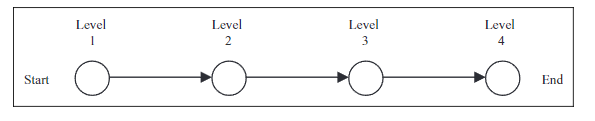
\includegraphics[width=\textwidth]{ch2_1_linear.png}
    \caption{Liniowa struktura gry\cite{narrative_structures}}
    \centering
    \label{fig:ch1_2_1_linear}
\end{figure}

\subsection{Łańcuch pereł}

W ramach tego modelu gracze uzyskują pewnego rodzaju \textit{"iluzję"} wyboru. Występują podczas
rozgrywki momenty swobody, gdzie grający mają poczucie wpływu na dalszy przebieg fabularny. W
rzeczywistości jednak podejmowane przez nich decyzje mogą nie posuwać historii na przód, a same
postępy narracyjne nadal znajdują się pod kontrolą projektantów gry\cite{theorising_narrative}.
Tak jak przedstawiono na rysunku \ref{fig:ch1_2_1_pearls} --- mogą występować tymczasowe rozgałęzienia
wychodzące od głównej sekwencji fabularnej, natomiast zostają one w końcu urwane, a gracz zobowiązany
jest do kontynuowania przygody według zaplanowanej historii. Jako przykład może służyć "The Legend
of Zelda" (Patrz \ref{subsection:ch1_2}), gdzie grający może zwiedzać dane poziomy w dość dowolny
sposób, natomiast musi ostatecznie trafić na główną ścieżkę by móc dokonać postępu.

\begin{figure}[h]
    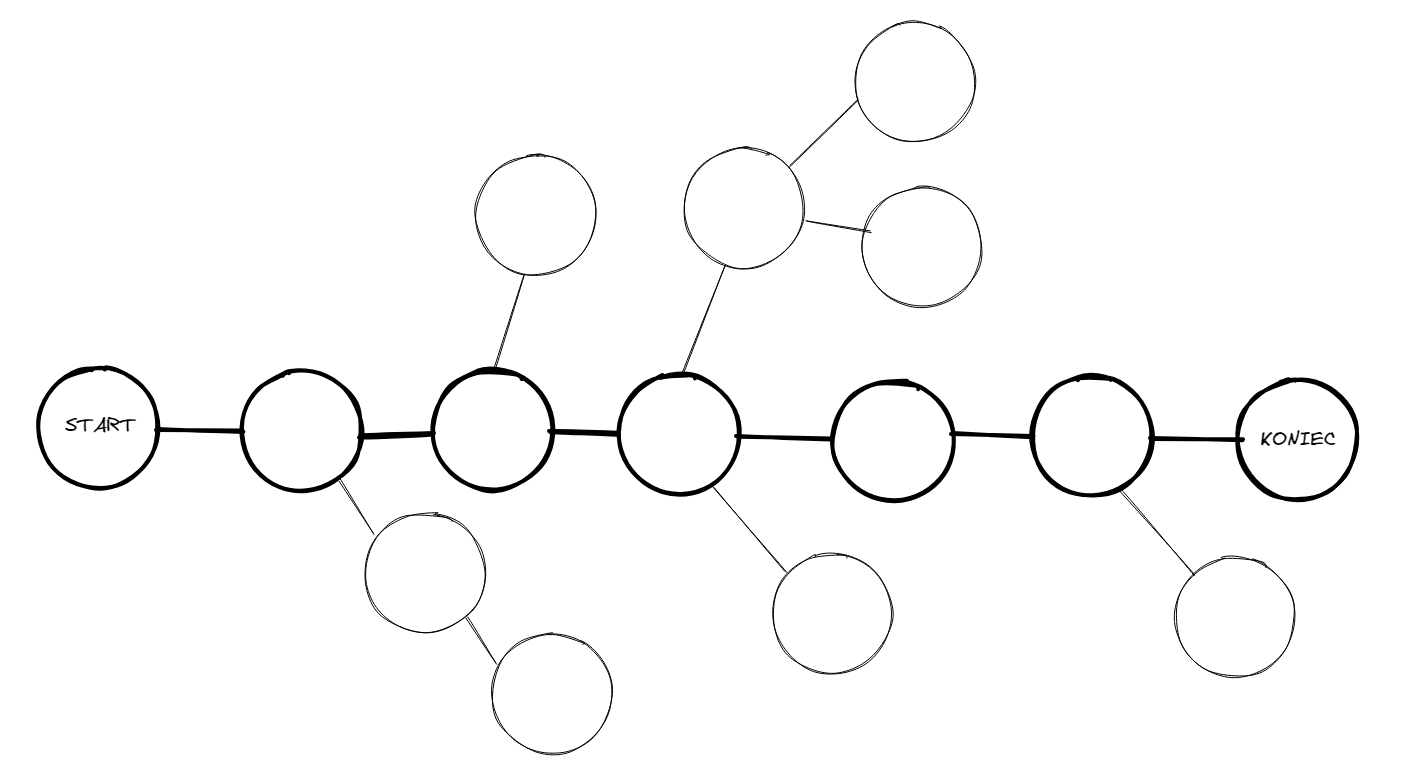
\includegraphics[width=\textwidth]{ch2_1_pearls.png}
    \caption{Struktura łańcuchu pereł}
    \centering
    \label{fig:ch1_2_1_pearls}
\end{figure}

\subsection{Rozgałęziająca się}

Metodą, która oferuje graczowi istotny wpływ na przebieg dalszej rozgrywki jest zdecydowanie
model rozgałęziający się. Jak sama nazwa wskazuje, historia nie trzyma się jednej konkretnej wersji
lecz jest w stanie \textit{"rozgałęziać się"} w wielu innych możliwych kierunkach. Może to wynikać
z jawnych decyzji podejmowanych przez gracza w istotnych momentach lub też ze względu na sposób
w jaki podchodzi on do rozgrywki (np. może pomijać pewne elementy świata)\cite{theorising_narrative}.
W wyniku takich rozgałęzień wytwarza się pewnego rodzaju "sieć możliwości fabularnych"\cite{theorising_narrative}
--- które z reguły muszą być uprzednio przygotowane przez projektantów gry. Struktura ta została
przedstawiona na rysunku \ref{fig:ch1_2_1_branching} --- akcja zaczyna się w jednym punkcie, potem
w wyniku decyzji istniejących w grze występują rozgałęzienia, które ostatecznie prowadzą do potencjalnie
różnych zakończeń (oznaczonych czerwonymi rombami). Przykładem realizującym ten model może być
wspomniany wcześniej tytuł "Life is Strange" (Patrz \ref{subsection:ch1_2}).

\begin{figure}[h]
    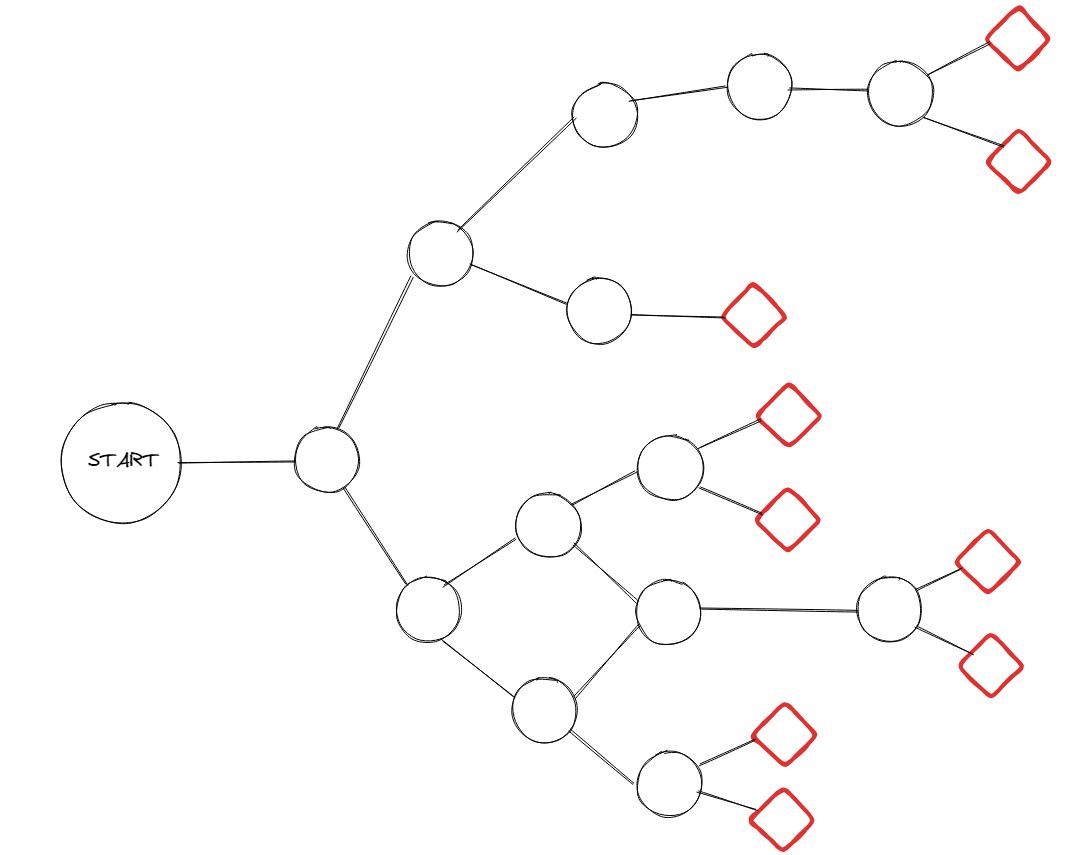
\includegraphics[width=\textwidth]{ch2_1_branching.png}
    \caption{Struktura rozgałęziająca się}
    \centering
    \label{fig:ch1_2_1_branching}
\end{figure}

\newpage

\subsection{Park rozrywki}

Struktura ta z założenia bardzo przypomina model rozgałęziający się, natomiast w tym przypadku
możemy mówić o narracji rozwijającej się ze względu na przestrzeń a nie czas\cite{theorising_narrative}.
Przykładowo, zwiedzając świat gry gracz może napotkać postać \gls{npc}, która otworzy przed nim nową
gałąź fabularną (np. poprzez zlecenia zadania do wykonania)\cite{the_evolution_of_video_games}.
Model ten jest bardzo popularny dla gier z otwartym światem, przykładem może być "Wiedźmin 3"
(Patrz \ref{subsection:ch1_2}).

\subsection{Cegiełki}

W ramach niektórych tytułów twórcy nie skupiają się na stworzeniu narracji możliwej do doświadczenia
przez grającego, lecz na pewnym systemie części, za pomocą których gracz sam jest w stanie tworzyć
historię. Części te nazywane \textit{"cegiełkami"} (ang. \textit{building blocks})\cite{theorising_narrative}
są wykorzystywane przez grającego do tworzenia własnej narracji. Przykładem tego rodzaju rozgrywki
może być tytuł "The Sims" (2000), w którym to gracz tworzy i steruje rodziną --- a co za tym idzie,
kieruje ich historią życia.

\section{Sposoby przedstawiania narracji}\label{subsection:ch1_2_2}

Oprócz zaplanowania i rozłożenia fabuły gry na części --- przy użyciu kombinacji struktur opisanych
w poprzedniej sekcji --- istotną kwestią pozostaje wybór w jaki sposób dane sekwencje fabularne
mają zostać przekazane graczowi. W ramach tej sekcji opisane zostaną najważniejsze techniki
prezentowania narracji.

\subsection{Cut scenki}\label{subsubsection:ch1_2_2_cutscene}

Jednym z najbardziej widowiskowych sposobów prezentowania treści fabularnej jest zdecydowanie
cut scenka, która zdefiniowana została przez Glassnera (2004) następująco:

\begin{quotation}
    \textit{... pre-renderowany fragment wideo ... czasami renderowany w czasie rzeczywistym przy
        użyciu sprzętu komputerowego lub konsoli. Podczas odtwarzania możliwość interakcji gracza
        zostaje zawieszona, a on sam staje się biernym widzem na czas trwania sceny}\cite{narrative_structures}
\end{quotation}

Cut scenka jest zatem po prostu fragmentem wideo. Można dokonać pewnego podziału ze względu na
sposób renderowania czy też możliwość interakcji gracza (której powyższa definicja nie przewiduje).
W ramach materiału pre-renderowanego gracz obserwuje de facto odtwarzany plik wideo, który mógł
być wyprodukowany w dowolny sposób. Typowy silnik gry nie jest w tym momencie używany, a filmik
jest prezentowany w pewnego rodzaju odtwarzaczu multimedialnym. W przypadku materiału renderowanego
w czasie rzeczywistym wykorzystywany jest silnik gry oraz modele/tekstury występujące podczas
rozgrywki. Zapewnia to zdecydowanie płynniejsze przechodzenie pomiędzy momentami nieinteraktywnymi
i interaktywnymi oraz prowadzi do większej spójności wizualnej. Wymaganie użycia sprzętu komputerowego
może prowadzić do pewnego ograniczenia jakości czy też wykorzystywanych technik (jak np. symulacji
fizycznych). Klasycznie cut scenki nie są interaktywne a gracz jest jedynie pasywnym odbiorcą.
W niektórych tytułach możemy jednak natknąć się na metodę \gls{qte} (z ang. \textit{quick time event}), w
ramach której podczas odgrywania danej scenki wyświetlają się ikonki (potencjalnie wraz z instrukcjami)
symbolizujące przycisk do wciśnięcia przez gracza. Wymusza to na nim uważność przy oglądaniu materiałów
a dodatkowo wprowadza mechanizm stresowy, ponieważ często błędnie wykonane sekwencje pociągają
za sobą konsekwencje fabularne (np. śmierć danej postaci). Cut-scenki w wersji klasycznej jak i z
uwzględnieniem \gls{qte} zostały zaprezentowane na rysunku \ref{fig:ch1_2_2_cutscene}.

\begin{figure}[h]
    \begin{subfigure}{0.49\textwidth}
        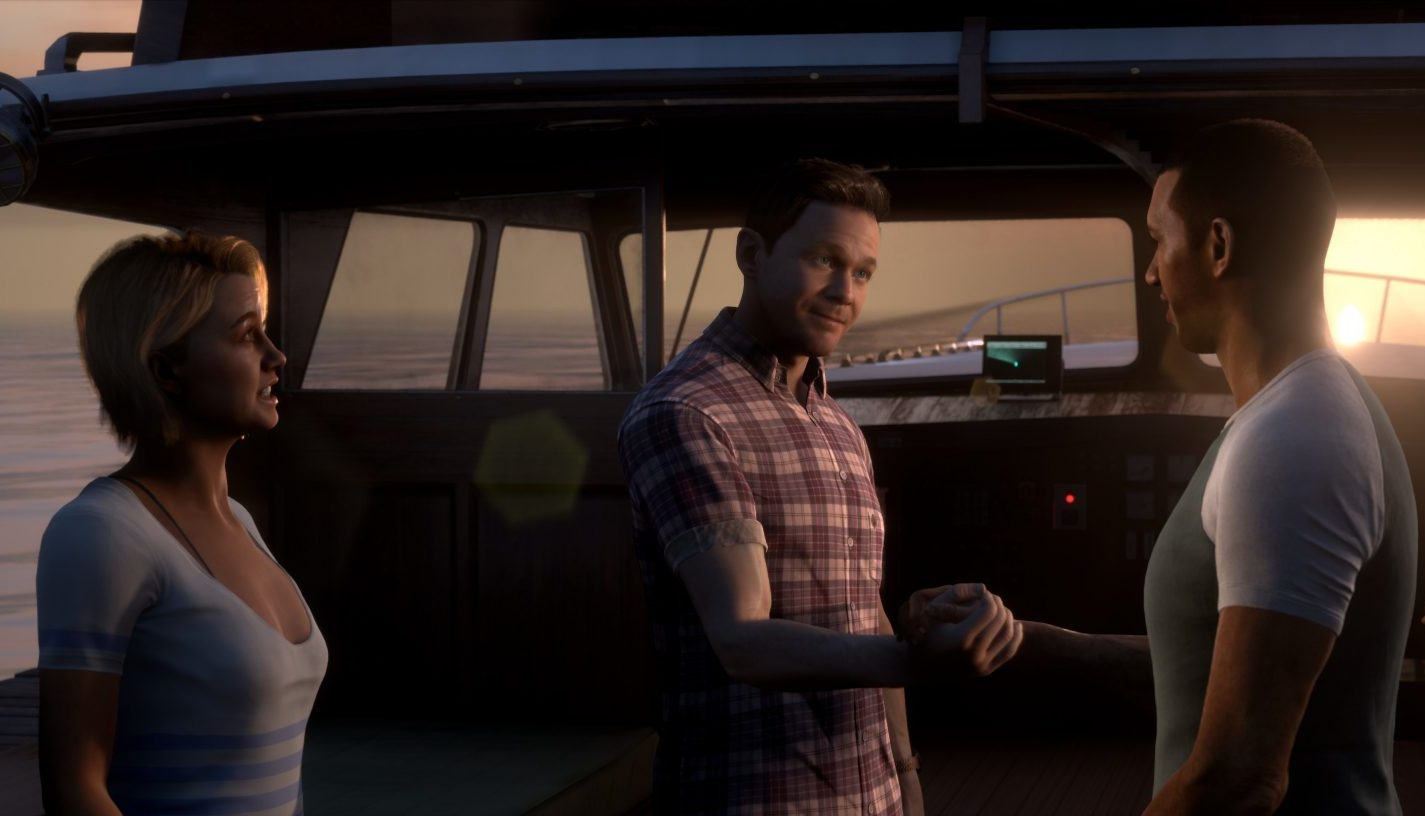
\includegraphics[width=\linewidth, height=6cm]{ch2_2_cutscene.jpg}
        \caption{Normalna cut-scenka}
        \label{subfig:ch2_2_cutscene1}
    \end{subfigure}
    \begin{subfigure}{0.49\textwidth}
        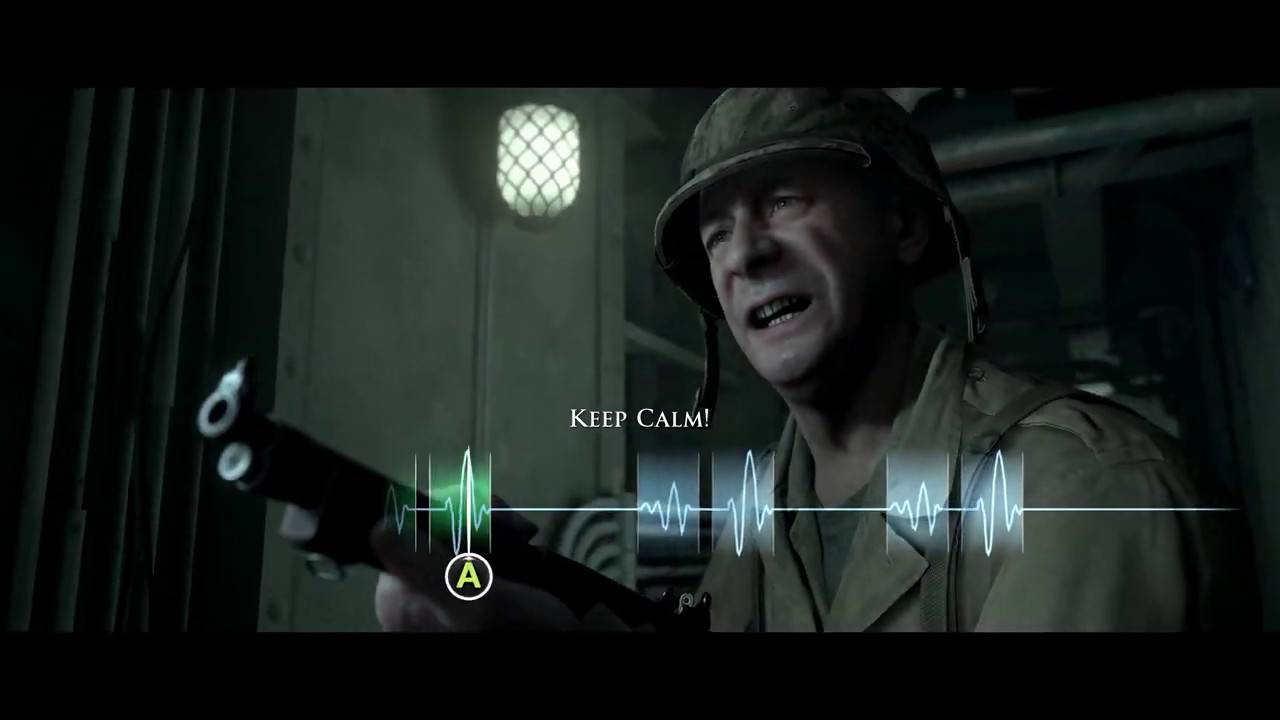
\includegraphics[width=\linewidth, height=6cm]{ch2_2_cutscene2.jpg}
        \caption{Cut-scenka z \gls{qte}}
        \label{subfig:ch2_2_cutscene2}
    \end{subfigure}
    \caption{The Dark Pictures Anthology: Man of Medan (2019) - Supermassive Games}
    \label{fig:ch1_2_2_cutscene}
\end{figure}

\newpage

\subsection{Tekst}

W przypadku tekstu możemy mówić o pełnoprawnych blokach tekstowych (Rys. \ref{fig:ch1_2_2_text}),
elementach interfejsu czy też o odpowiednich komunikatach pojawiających się na ekranie. Jest to
oczywiście bardzo prosta forma przekazu fabularnego, wzorująca się na szeroko pojętej literaturze.
Może być wykorzystany jako główny sposób prowadzenia opowieści lub jako element pomocniczny, często
robiący fabularnie sens (np. w "Final Fantasy XIII" postacie naturalnie prowadzą między sobą dialog,
ale informacje o świecie skryte w formie notatek znajdowanych przez gracza w trakie rozgrywki).

\begin{figure}[h]
    \begin{subfigure}{0.49\textwidth}
        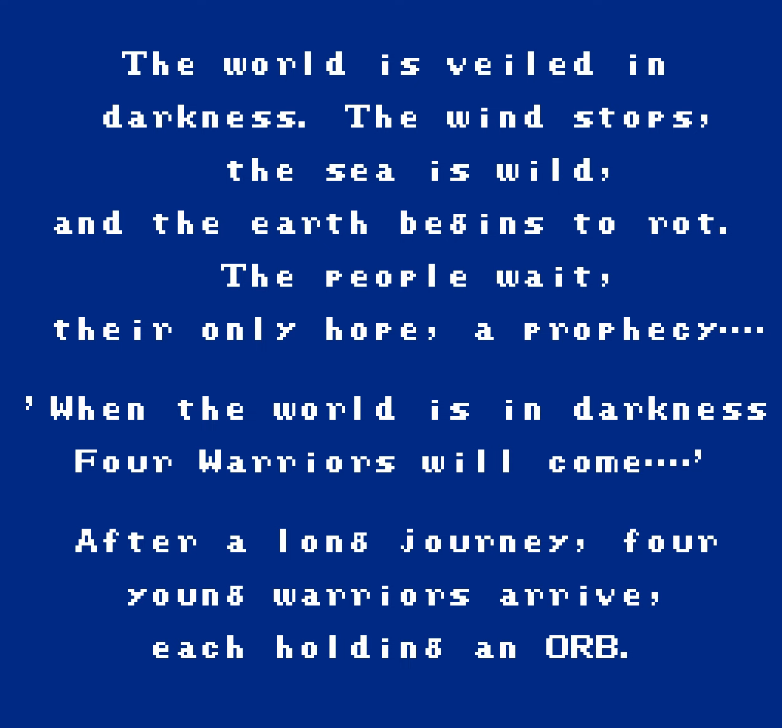
\includegraphics[width=\linewidth, height=6cm]{ch2_ff1.png}
        \caption{Final Fantasy I (1987)}
        \label{subfig:ch2_2_text1}
    \end{subfigure}
    \begin{subfigure}{0.49\textwidth}
        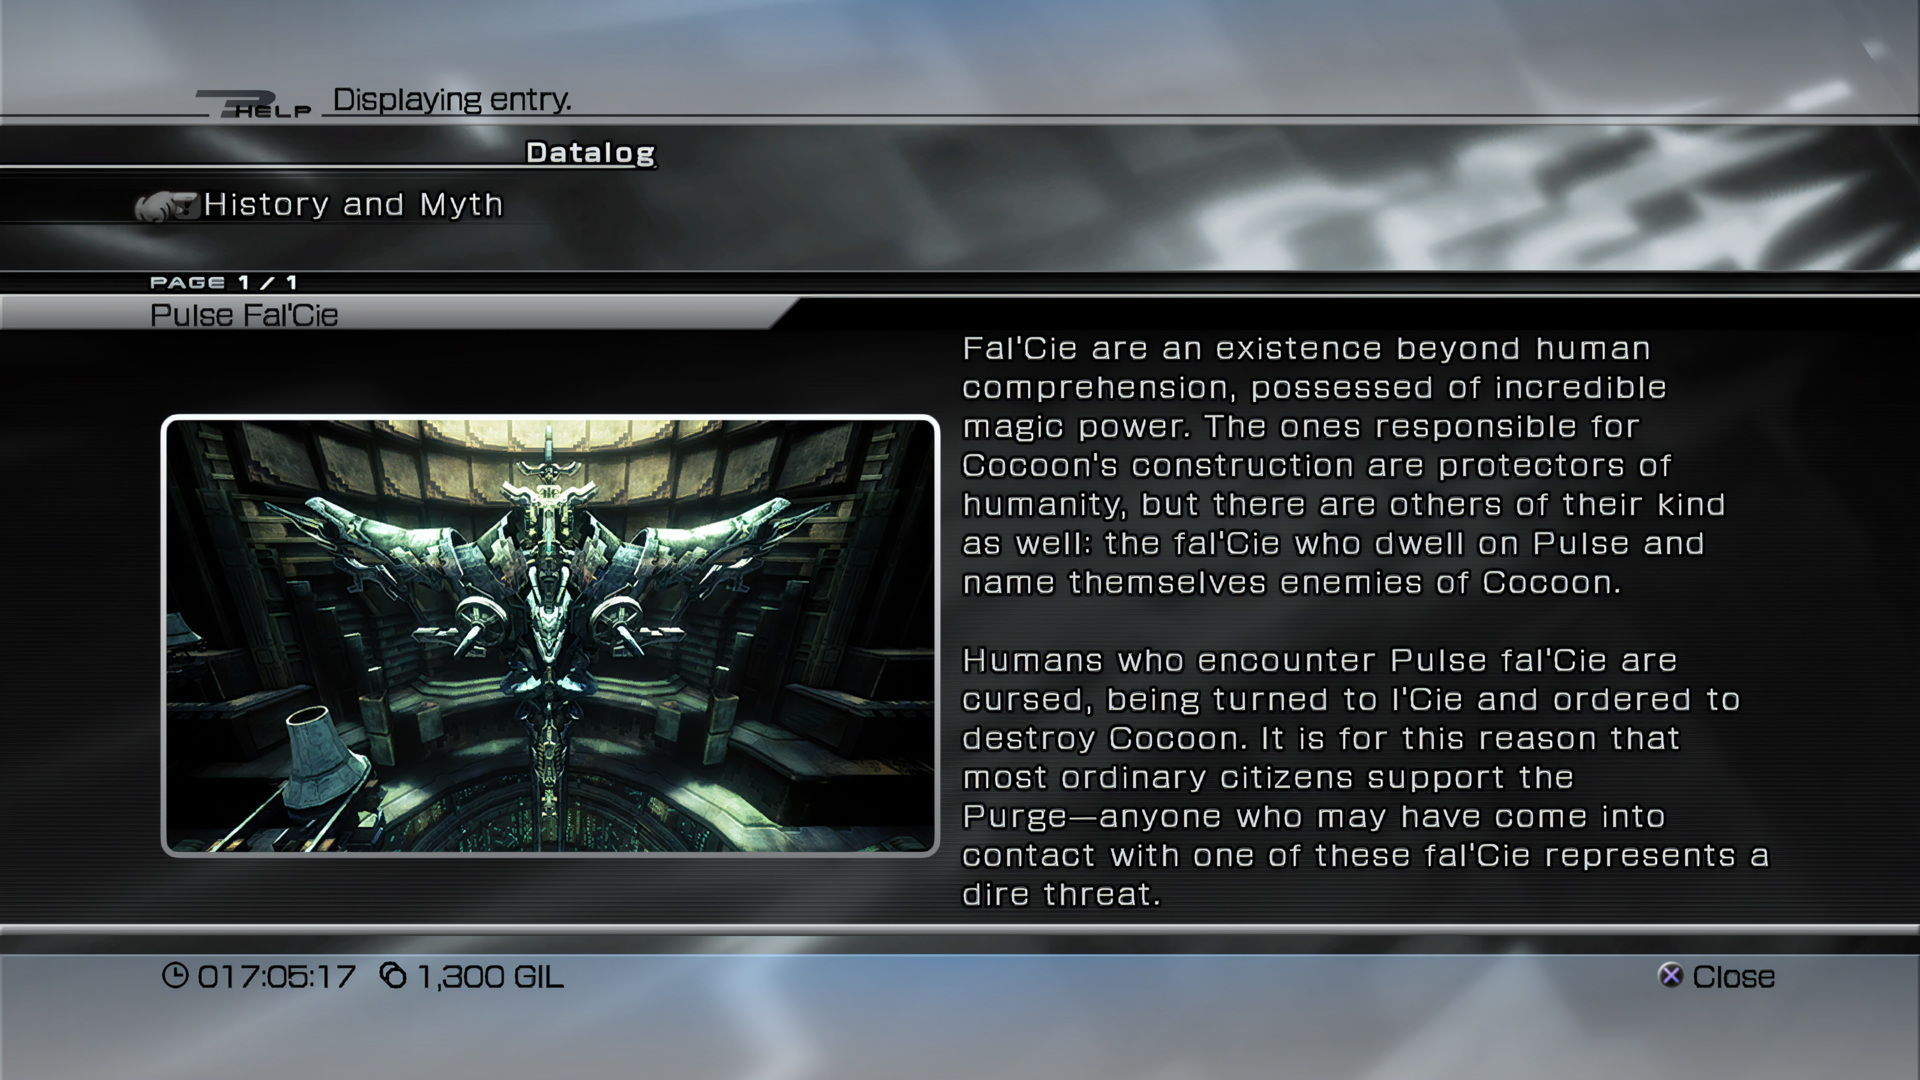
\includegraphics[width=\linewidth, height=6cm]{ch2_ff13.png}
        \caption{Final Fantasy XIII (2009)}
        \label{subfig:ch2_2_text2}
    \end{subfigure}
    \caption{Bloki tekstu służące do przedstawienia fabuły}
    \label{fig:ch1_2_2_text}
\end{figure}

\subsection{Dialogi (głównie z NPC)}

Dialog jako forma przedstawienia narracji może stanowić połączenie tekstu, dźwięku, animacji i
interaktywności. Tekst może być obecny w formie napisów pomocniczych do kwestii wypowiadanych przez
postacie, ale i również prezentuje możliwości do wyboru dostępne dla gracza. Współcześnie wiele gier
nadaje głos swoim postaciom przy pomocy aktorów głosowych. Tak jak w przypadku cut scenek w czasie
rzeczywistym, postacie najczęściej są animowane podczas dialogu, korzystając z silnika gry.
Interaktywność podczas dialogu może wyłaniać się w formie przeklikiwania kolejnych kwestii (by dać
graczowi czas na przeczytanie / zastanowienie się) lub poprzez możliwość wyboru kolejnych kwestii.
W zależności od tytułu niektóre konwersacje mogą przypominać strukturę łańcucha pereł (gdzie
rozmowa i tak kończy się w ten sam sposób) a niektóre formę rozgałęziającą się (gdzie odpowiedni
wybór może nieść za sobą dalsze konsekwencje fabularne) [Patrz \ref{subsection:ch1_2_1}]. Więcej
o systemach dialogowych wspomniane jest w sekcji \ref{subsection:ch3_1}.

\begin{figure}[h]
    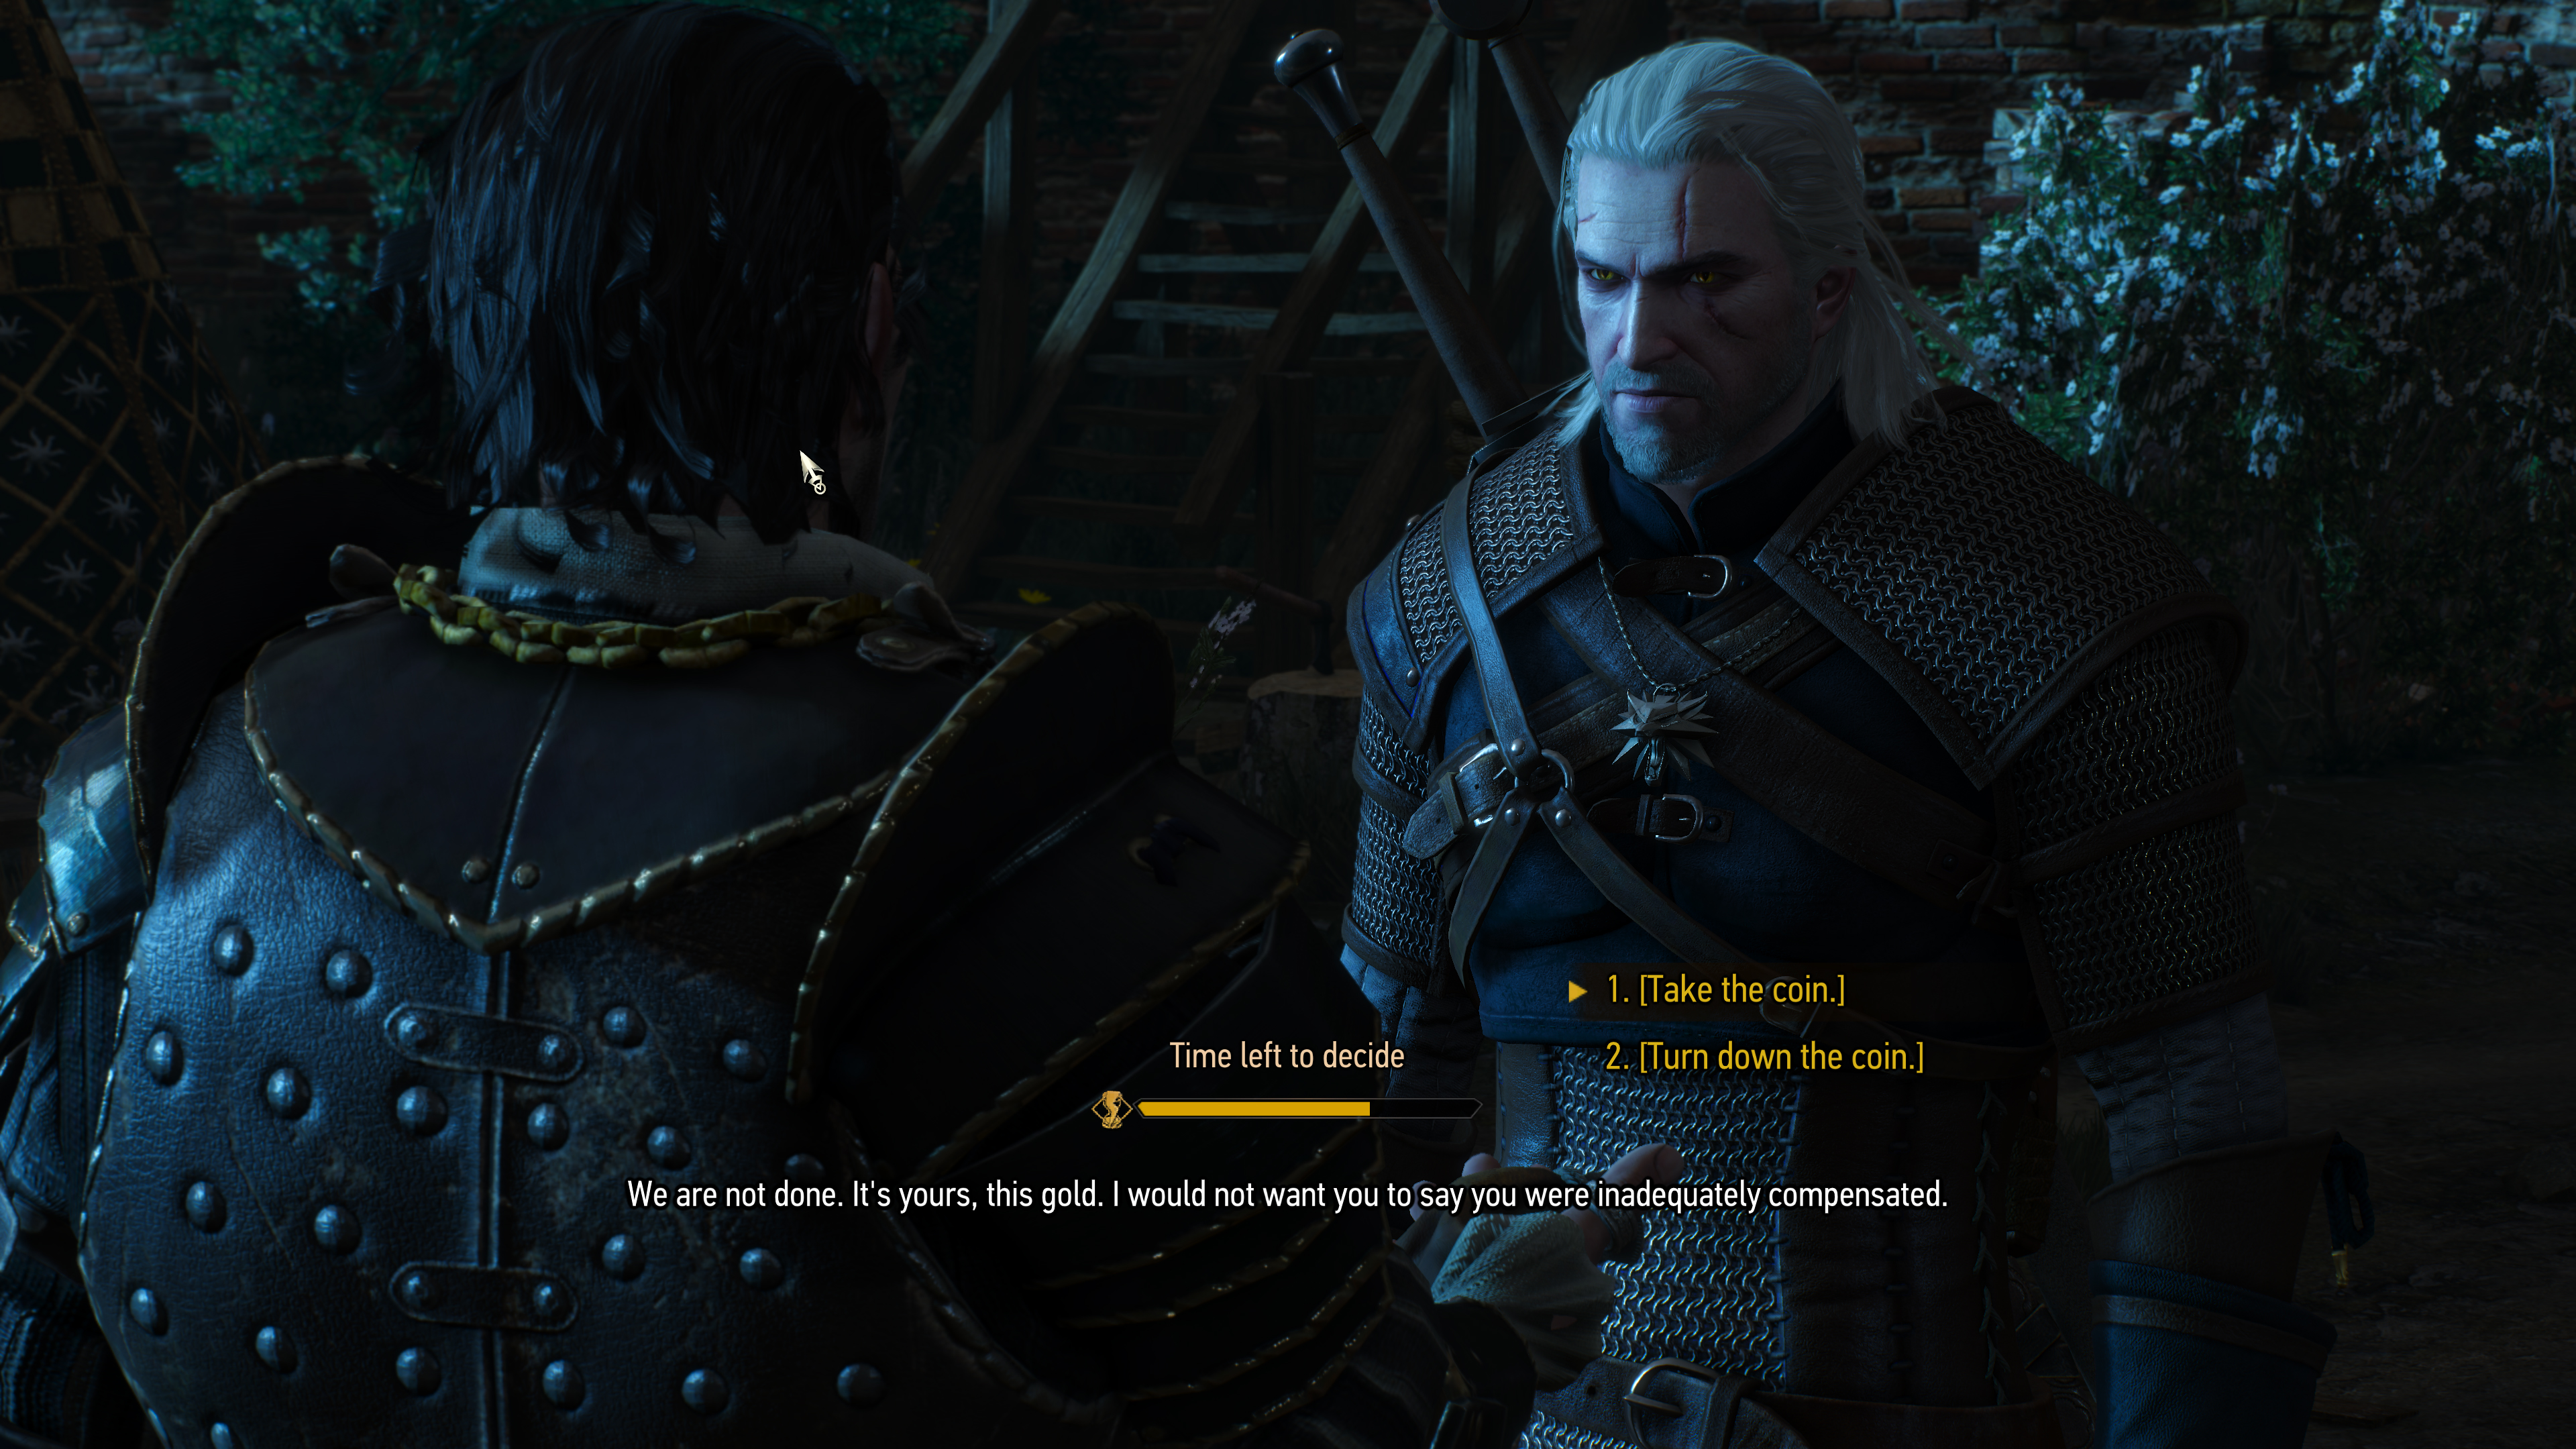
\includegraphics[width=\textwidth]{ch2_witcher_2.png}
    \caption{Dialog z \gls{npc} - "Wiedźmin 3" (2015)}
    \centering
    \label{fig:ch1_2_2_dialogue}
\end{figure}

\subsection{Poprzez świat gry (audio-wizualne)}

Najciekawszym a zarazem najrzadszym\cite{the_evolution_of_video_games} sposobem prezentowania fabuły
jest opowiadanie za pomocą samego świata gry. Mowa tu o obiektach i ich umiejscowieniu, teksturach,
ścieżkach dźwiękowych czy wszelkich innych widocznych lub słyszalnych elementach świata. Jedną z
serii gier, która bazuje na tym koncepcie i cieszy się ogromną popularnością, jest "Dark Souls".
Cut scenki są bardzo sporadyczne, przeważnie na początku i końcu rozgrywki oraz prezentujące starcie
z trudnymi przeciwnikami (\textit{"bossami"}). Spotykane postacie \gls{npc} są bardzo enigmatyczne, nie
zadają graczowi wprost zadań do wykonania i posiadają tylko kilka zapętlających się kwestii
dialogowych. Tekstowy opis dotyczy głównie znajdowanych przedmiotów i zawiera szczątkowe informacje
dotyczące ogólnopojętego świata gry. W ten sposób gracz musi samemu układać fabułę, na podstawie
znajdowanych skrawków wiedzy. Dodatkowo, muzyka występuje tylko w ramach pojedynczych lokacji albo
w przypadku starć z \textit{"bossami"}. W ten sposób autorzy podkreślają wagę tego co jest właśnie
prezentowane na ekranie i starają się wywołać u gracza pewne emocje.